\documentclass[11pt]{article}

% Packages for math and proof writing
\usepackage{amsmath, amssymb, amsthm}
\usepackage{bbm}

% Theorem and proof environments
\newtheorem{theorem}{Theorem}
\newtheorem{lemma}[theorem]{Lemma}
\newtheorem{proposition}[theorem]{Proposition}
\newtheorem{corollary}[theorem]{Corollary}

% Definitions, remarks, etc.
\theoremstyle{definition}
\newtheorem{definition}[theorem]{Definition}
\newtheorem{example}[theorem]{Example}

\theoremstyle{remark}
\newtheorem{remark}[theorem]{Remark}

% Page formatting
\usepackage[margin=1in]{geometry}

%tikz formatting

\usepackage{tikz}
\usetikzlibrary{patterns} % for patterns like checkerboard or hatchings
\usepackage{caption}
\usepackage{url}

\title{Week 9:\ Probability Theory}
\author{David Kinney}
\date{October 23rd, 2025}

\begin{document}

\maketitle

\section{Introduction}
Throughout the sciences, probability theory is used extensively to measure both uncertainty about the state of the world and inherent indeterminacy in the systems that generate the data that we observe. Thus, it is not surprising that probability theory, perhaps more than any other area of mathematics, is deployed regularly in philosophy, especially in epistemology and philosophy of science. Across philosophy, uses of probability theory codomain from the very casual to the very rigorous. The goal of this reading is to provide a reasonably rigorous introduction to the most important parts of probability theory as it is used in philosophy, before moving on to some explicit discussion of the two major ways that probability is used in philosophy.\par

The material in Sections \ref{subsec:count} and \ref{subsec:uncount} is pretty dense. There won't be any problem set questions that depend on it, so you can skip it if you'd like. But I think it's highly advisable to have a look at those sections at some point if you want to use probability theory in your research work.\par 


\section{Probability Spaces}
The most important concept in probability theory is the concept of the \textbf{probability space}. A probability space is a triple $(\Omega,\Sigma,p)$, where $\Omega$ and $\Sigma$ are sets and $p$ is a function. The set $\Omega$ is called the \textbf{sample space} (or, sometimes, the \textbf{state space)}, the set $\Sigma$ is called the \textbf{$\sigma$-algebra}, and the function $p$ is a called the \textbf{probability distribution}.\par

The sample space $\Omega$ is a set whose elements represent the most fine-grained set of possibilities that we might wish to consider in a particular application of probability theory. Often, it will make sense to think of $\Omega$ as the set of all possible worlds, but, depending on what one is using probability theory to do, one can alternative think of $\Omega$ as the set of all relevant scenarios an agent might find themselves in, or the set of all states that a system might be in. For the rest of this reading, I will usually treat $\Omega$ as the set of all possible worlds, but I want to be careful to note that this is only an \textit{interpretation} of $\Omega$ that characterizes a particular application of probability theory, rather than a requirement of probability theory itself.\par 

The $\sigma$-algebra $\Sigma$ is a set of subsets of $\Omega$ that satisfies the following individually necessary and jointly sufficient conditions:
\begin{itemize}
    \item $\emptyset\in\Sigma$

    \item $\Omega\in\Sigma$

    \item $\Sigma$ is \textbf{closed under complement}. This means that if $A\in \Sigma$, then $(\Omega\setminus A)\in \Sigma$.

    \item $\Sigma$ is \textbf{closed under countable union}. This means that if $\mathcal{A}$ is a set of subsets of $\Omega$ with countable cardinality (i.e., its cardinality is finite or countably infinite) and $\cup\mathcal{A}$ is the set of all elements of any element of $\mathcal{A}$ (i.e., the union of all elements of $\mathcal{A})$, then $\cup A\in \Sigma$.

    \item $\Sigma$ is \textbf{closed under countable intersection}. This means that if $\mathcal{A}$ is a set of subsets of $\Omega$ with countable cardinality  and $\cap\mathcal{A}$ is the set of all elements of all elements of $\mathcal{A}$ (i.e., the intersection of all elements of $\mathcal{A})$, then $\cap A\in \Sigma$.
\end{itemize}
For any $\Omega$, its power set $\mathcal{P}(\Omega)$ is a $\sigma$-algebra. However, for many $\Omega$, we can also define a $\sigma$-algebra $\Sigma$ that is that a proper subset of the power set of $\Omega$ (i.e., $\Sigma\subset\mathcal{P}(\Omega)$). For example, consider the set of natural numbers $\mathbbm{N}$. Let $E$ be the set of all even natural numbers and let $O$ be the set of all odd natural numbers. One can easily check that the following set is a $\sigma$-algebra with respect to $\mathbbm{N}$:\ $\{\emptyset,E,O,\mathbbm{N}\}$. However, while this set is clearly a proper subset of the power set $\mathcal{P}(\mathbbm{N})$, it is not identical to $\mathcal{P}(\mathbbm{N})$. This point becomes especially important when $\Omega$ has uncountable cardinality; we will return to it shortly.\par 

If $\Omega$ is interpreted as the set of all possible worlds, then one can think of $\Sigma$ as a set of events that might occur. For example, the event that it rains in St.\ Louis on October 16th, 2025 is just the set of possible worlds where it rains in St.\ Louis on October 16th, 2025. This is why $\Sigma$ is sometimes called the ``event algebra.'' One can also take the proposition `it will rain in St.\ Louis on October 16th, 2025' to be represented by the set of possible worlds where it rains in St.\ Louis on October 16th, 2025. Under this interpretation, $\Sigma$ is the set of all propositions that can be assigned probabilities.\par

This leaves the probability distribution $p$. To define this distribution, let $[0,1]$ be the set of all real numbers greater than or equal to zero or less than or equal to one. The probability distribution $p$ is a function $p:\Sigma\rightarrow[0,1]$ (i.e., a function assigning events or propositions a number between $0$ and $1$, inclusive) that satisfies the following three properties:
\begin{enumerate}
    \item $p(\Omega)=1$.

    \item For all $A\in\Sigma$, $p(A)\geq 0$.
    
    \item For any $\mathcal{A}\subset\Sigma$ with countable cardinality such that for any $A\in\mathcal{A}$ and $A^{\prime}\in\mathcal{A}$, $A\cap A^{\prime}=\emptyset$, $$p(\cup\mathcal{A})=\sum_{A\in\mathcal{A}}p(A).$$ 
\end{enumerate}
One should read the right-hand side of the equation above as `the sum of each $p(A)$ for all $A\in\mathcal{A}$.' These three properties are known as \textbf{Kolmogorov's axioms}, after Audrey Kolmogorov (1903-1987), who is credited as the founder of modern probability theory. The first axiom effectively says that the probability that \textit{some} event happens is one. The second axiom says that all probabilities are non-negative. The third axiom says that the probability of the union of any countable set of mutually disjoint events (i.e., events that do not share any possible worlds with each other) is equal to the sum of probabilities assigned to each disjoint event.\par

As a simple example, suppose that $\Omega=\{1,2,3,4,5,6\}$, representing six possible outcomes of a die roll. Let $\Sigma$ be the power set of $\Omega$. For any $A\in\Sigma$, $p(A)$ is the probability of obtaining any number in $A$ when rolling the die. The first of Kolmogorov's axioms, $p(\Omega)=1$, states that the probability that the die roll yields a number from one to six is one. The second axiom states that no probabilities are negative. The third probability tells us that, for example, the probability $p(\{1,4\})$ that the die roll yields a one or a four is given by the sum $p(\{1,4\})=p(\{1\}) + p(\{4\})$.\par

The Kolmogorov axioms are surprisingly powerful; all of probability theory is built off of them. As just one small example, consider the following proposition:
\begin{proposition}
    For any probability space $(\Omega,\Sigma,p)$, $p(\emptyset)=0$.
\end{proposition}
\begin{proof}
    From the first Kolmogorov axiom, we have $p(\Omega)=1$. Note that $\Omega\cap\emptyset=\emptyset$. Thus, it follows from the third Kolmogorov axiom that $p(\emptyset)+p(\Omega)=p(\Omega)$. Substituting $1$ for $p(\Omega)$ gives us $p(\emptyset)+1=1$. It follows that $p(\emptyset)=0$.
\end{proof}
\noindent
This proof is an example of the style of proof I'm looking for in the problem set for this week:\ it convinces the reader of what is to be proved in a wholly general way, but is still written in a prose style rather than a numbered list of propositions.\par 

Earlier, I mentioned that when $\Omega$ has uncountable cardinality, the fact that we can define $\sigma$-algebras that are \textit{not} the power set of $\Omega$ is important. Let me now be clear as to why this fact becomes important in this context. Suppose that $\Omega=\mathbbm{R}$. In 1905, Guiseppe Vitali (1875-1932) proved that, under the assumption that the axiom of choice holds, if $\Sigma$ is the power set of $\mathbbm{R}$, then there is no probability distribution $p:\Sigma\rightarrow[0,1]$ that, in addition to satisfying Kolmogorov's three axioms, also has the following property:
\begin{quote}
\textbf{Translation Invariance:\ }$p(A) = p(\{a+x:a\in A\})$ for any $A\in\Sigma$ and $x\in\mathbbm{R}$.
\end{quote}
However, translation invariance seems to be an intuitively desirable property for any ``uniform'' probability distribution on the real numbers. All it says is that if some set of real numbers $A$ has probability $p(A)$, then a set $A^{\prime}$ that is generated by adding the same number to every real number in $A$ should be such that $p(A^{\prime})=p(A)$.  Moreover, the axiom of choice is needed for a lot of the things we want to do with probability. So, the fact that, under the axiom of choice, no probability distribution whose domain is the power set of the real numbers can satisfy translation invariance is generally taken to show that when $\Omega$ is of uncountable cardinality, the power set $\mathcal{P}(\Omega)$ is not a ``well-behaved'' sigma-algebra that can serve as the domain of a probability distribution. Instead, when $\Omega$ is of uncountable cardinality, we typically form a probability space $(\Omega,\mathcal{B},p)$, where $\mathcal{B}\subset\mathcal{P}(\Omega)$ is a specially-defined $\sigma$-algebra called the \textbf{Borel $\sigma$-algebra} after \'Emile Borel (1871-1956). To grasp the significance of the Borel $\sigma$-algebra, begin by considering the following two facts:\
\begin{enumerate}
    \item An \textbf{open set} of real numbers is a set $S\subseteq\mathbbm{R}$ such that for any $x\in S$, there is some $\epsilon>0$ such that all real numbers between $x-\epsilon$ and $x+\epsilon$ are in $S$. The Borel $\sigma$-algebra contains all open subsets of the real numbers.
    
    \item An \textbf{closed set} of real numbers is a set $S\subseteq\mathbbm{R}$ such that its complement $\mathbbm{R}\setminus S$ is an open set The Borel $\sigma$-algebra contains all closed subsets of the real numbers.
\end{enumerate}
In addition, we can define a probability distribution on the Borel $\sigma$-algebra that satisfies translation invariance. Thus, if we think of an accountable sample space $\Omega$ as an uncountable set of possible worlds, and if we think of the set of all possible events as the set of open or closed possible worlds, then the Borel $\sigma$-algebra provides a well-behaved algebra of events.\par 


The definition of the Borel $\sigma$-algebra is complicated, and we won't go over it here. Nevertheless, its existence is important for at least two reasons. First, in philosophical uses of probability theory one often wishes to use an uncountable sample space $\Omega$. For example, one often wishes for the sample space to be the set of all possible worlds, and there are many good reasons to think the set of all possible worlds has uncountable cardinality. In such a case, one must be careful to use a well-behaved $\sigma$-algebra like the Borel $\sigma$-algebra. Second, when we discuss null-hypothesis significance testing next week, we will have to mention the Borel $\sigma$-algebra again. 


\section{Conditional Probability}
Consider any probability space $(\Omega,\Sigma,p)$ and any $A\in\Sigma$ and $B\in\Sigma$. The probability that $A$ occurs, given that $B$ is true, is denoted $p(A|B)$. In general, $p(A|B)$ is related to the probabilities $p(A\cap B)$ and $p(B)$ via the following formula, which I will call the \textbf{basic constraint} (this is not a standard term):
$$p(A|B)p(B) = P(A\cap B).$$
When $p(B)\geq 0$, the basic constraint allows us to derive an equation for computing the value of $p(A|B)$ standardly known as the \textbf{ratio formula}:\ 
$$p(A|B) = \frac{p(A\cap B)}{p(B)}.$$
To grasp the intuition behind the ratio formula, consider the Venn diagram in Fig.~\ref{fig:vennAB}.\footnote{The Venn diagram was invented by the British mathematician and philosopher John Venn (1834-1923).} Suppose that we are randomly going to select a point from within the box. Suppose that the probability of a point falling in any region of the box is given by the area of that region. Given that the point we select is necessarily going to be in $B$, what is the probability that the probability that the point also falls in the checkered region representing the overlap between $A$ and $B$? The intuitive answer, encoded in the ratio formula, is that it is the proportion of the area of $B$ that is also part of the area of $A$. For example, if the checkered region takes up 30\% of the area of circle the represents the set $B$, then the probability of a randomly selected point being in the checkered region, given that it is necessarily in $B$, is $.3$.

\begin{figure}[]
\centering
\fbox{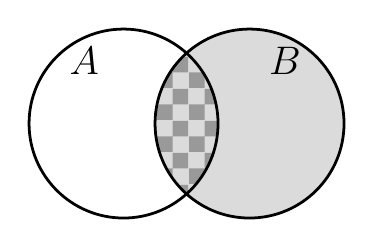
\begin{tikzpicture}[scale=1]
  % circle centers and radius
  \def\R{1.2}
  \def\dx{0.8} % half-distance between centers

  % Circle B (right) shaded gray with some transparency
  \fill[gray!40, opacity=0.7] (\dx,0) circle (\R);

  % Intersection (A ∩ B) semi-transparent checker pattern
  \begin{scope}
    \clip (-\dx,0) circle (\R); % restrict to inside A
    \fill[pattern=checkerboard, pattern color=black, opacity=0.3] (\dx,0) circle (\R);
    % If checkerboard pattern not available, uncomment:
    % \fill[pattern=north east lines, pattern color=black, opacity=0.4] (\dx,0) circle (\R);
  \end{scope}

  % Circle A (left) outline
  \draw[line width=1pt] (-\dx,0) circle (\R);
  % Circle B (right) outline
  \draw[line width=1pt] (\dx,0) circle (\R);

  % Labels
  \node at (-\dx-0.5, .8) {\Large $A$};
  \node at (\dx+0.45, .8) {\Large $B$};

\end{tikzpicture}}
\caption{Venn Diagram.}
\label{fig:vennAB}
\end{figure}


Noting that the basic constraint can be used to derive $p(A\cap B)=p(B|A)p(A)$, the ratio formula can be re-written as the equation standardly known as \textbf{Bayes' theorem}, named after Thomas Bayes (1701-1761):
$$p(A|B) = \frac{p(B|A)p(A)}{p(B)}.$$
This equation will play an important role in our discussion of Bayesian statistics in two weeks.\par 

What happens when $p(B)=0$? Clearly, the ratio formula is undefined. Moreover, since $p(B)$ entails that $p(A\cap B)=0$, the basic constraint would seem to allow any probability for $p(A|B)$. But this doesn't mean that the notion of the probability of some event $A$ occurring, given that some event $B$ with probability $0$ has occurred, is meaningless. This is especially true when we consider probability spaces with an uncountable sample space. To see why, first consider the probability of selecting a single real number from the set of all real number $\mathbbm{R}$. We can represent this using a probability space $(\mathbbm{R},\mathcal{B},p)$, where $\mathcal{B}$ is the Borel $\sigma$-algebra on the real numbers. If we represent the probability of selecting a single real number $x\in\mathbbm{R}$ as $p(\{x\})$ and we want $p$ to satisfy translation invariance, then it \textit{must be the case }that $p(\{x\})=0$. Indeed, for a set of real numbers $S\subseteq\mathbbm{R}$ to have positive probability according to a translation-invariant probability distribution, then $S$ \textit{must} have uncountable cardinality. In a sense, this is what we want:\ if we want the probability of picking a finite subset of real numbers to be equal to the \textit{length} of that subset in the real number line, then any countable set of individual points has length zero, and so it should have probability zero. This case should drive home a crucial point about probability:\ \textit{in many cases, an event's having probability zero is not the same as it's being impossible.} I can imagine some quantity that can take any real number returning \textit{some} specific real number $x$ (i.e., $2$, or $\pi$, or $\sqrt{5}$), even though that outcome has probability zero. Indeed, none of these probability-zero outcomes seem impossible.\par

\begin{figure}[]
\centering
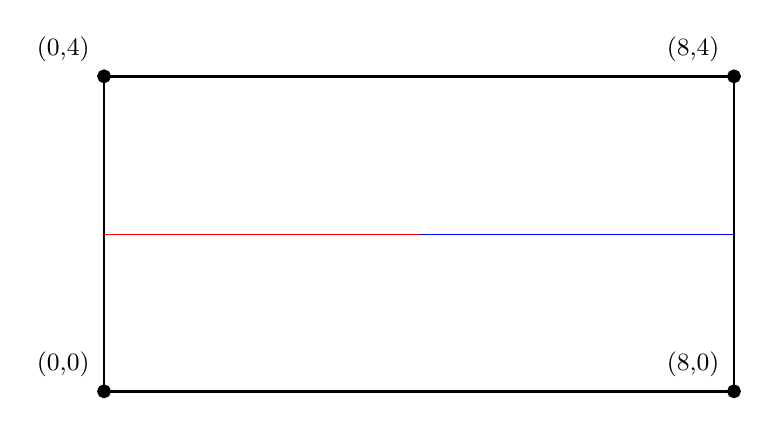
\begin{tikzpicture}[line width=1pt, scale=1]

  % Box dimensions
  \def\W{8} % width
  \def\H{4} % height

  % Draw outer box
  \draw[black] (0,0) rectangle (\W,\H);

  % Midpoint y-coordinate
  \def\Y{0.5*\H}

  % Horizontal line (half red, half blue)
  \draw[red, line width=.01pt] (0,\Y) -- (\W/2,\Y);
  \draw[blue, line width=.01pt] (\W/2,\Y) -- (\W,\Y);

  % Coordinates of the corners
  \foreach \x/\y in {0/0, \W/0, \W/\H, 0/\H} {
    \filldraw[black] (\x,\y) circle (2pt);
    \node[anchor=south east, font=\small] at (\x-0.05,\y+0.05) {(\x,\y)};
  }

\end{tikzpicture}
\caption{Example of Meaningfully Conditioning on a Probability-Zero Event}
\label{fig:box}
\end{figure}


Second, once we note that in the uncountable context probability-zero events are perfectly possible, there seem to be some intuitive answers to questions about what the conditional probability of some even is, given that some event with probability zero has occurred. To see this, consider the box in Fig.~\ref{fig:box}, whose corners sit at labeled coordinates. Suppose that the line running through the middle of the box represents just those points $(x,y)$ such that $y=2$. The portion of the line colored red represents just those points $(x,2)$ such that $x\geq0$ and $x\leq 4$, while the portion of the line colored blue represents just those points $(x,2)$ such that $x>4$ and $x\leq 8$. First we can ask, what is the probability that a randomly chosen point $(x,y)$ that is in the box falls on the line? If our sample space is the set of all points in the box and our event algebra is the Borel sigma algebra defined on that set, then for any translation-invariant probability distribution, the answer must be zero. However, suppose that a point \textit{did} fall on that line:\ what is the probability that it falls on the red half? The intuitive answer, it seems is $.5$:\ exactly half the line is red, so, given that a randomly chosen point is on the line, the probability that it is on the red half is $.5$.\par


Can we define conditional probability in such a way that it recovers these intuitions? Yes. Indeed, Kolmogorov's original treatment of conditional probability defined conditional probabilities in such a way that it doesn't matter if the probability of $p(B)=0$ when we define a conditional probability $p(A|B)$, with the ratio formula derived for the special case where $p(B)>0$.  However, I won't recapitulate it here, as the mathematics will take us a bit too far afield. One thing to note is that, in Kolmogorov's treatment, we need to make further assumptions about the probability distribution beyond his initial three axioms in order to derive a unique value for $p(A|B)$ in the case where $p(B)=0$. A really good introduction to Kolmogorov's original definition of conditional probability, which handles probability-zero cases, can be found in Kenny Easwaran's chapter ``Conditional Probability'' in the excellent \textit{Open Handbook of Formal Epistemology}, which you can get for free online at \url{https://philpapers.org/archive/PETTOH-2.pdf}.\par 


\section{Random Variables}
In many applications of probability, \textbf{random variables} (sometimes just called ``variables'') play an important role. To introduce random variables, consider any sample space $\Omega$. Let $\Sigma$ be any $\sigma$-algebra defined on $\Omega$ (i.e., its elements are all subsets of $\Omega$). The pair $(\Omega,\Sigma)$ is called a \textbf{measurable space}. A random variable is a function $V:\Omega\rightarrow\textsf{R}_{V}$, where $\textsf{R}_{V}$ is any set. A random variable is said to be \textbf{measurable} with respect to a measurable space $(\Omega,\Sigma)$ if, in addition to having $\Omega$ as its domain, for any $v\in\textsf{R}_{V}$, $V^{-1}(v)\in\Sigma$. To unpack this a bit, recall that, for any $v$ in the codomain of $V:\Omega\rightarrow\textsf{R}_{V}$, 
$$V^{-1}(v)=\{\omega\in\Omega:V(\omega)=v\}.$$
That is, the inverse $V^{-1}(v)$ is just the set of all elements of the sample space that the variable $V$ maps to the value $v$. When a random variable $V$ is measurable with respect to $(\Omega,\Sigma)$, it means that this set is in the event algebra $\Sigma$ for any value $v$ in the codomain of $V$.\par 


For any probability space $(\Omega,\Sigma,p)$, let $V$ be a random variable that is measurable with respect to $(\Omega,\Sigma)$. We are often interested in the probability that the variable $V$ takes some value $V$. We denote this probability $p(V=v)$. This probability is always given by the equation $$p(V=v)=p(V^{-1}(v)).$$ Since $V$ is measurable with respect to $(\Omega,\Sigma)$, we know that $V^{-1}(v)\in\Sigma$. Since $\Sigma$ is the domain of the probability distribution $p$, we know that $p(V^{-1}(v))$ will always have a specific value between $0$ and $1$, inclusive. Sometimes, we will have variables $X$ and $Y$ such that we are interested in the probability that $X$ takes some value $x$ and $Y$ takes some value $y$. We can calculate this \textbf{joint probability} via the formula $p(X=x,Y=y)=p(X^{-1}(x)\cap Y^{-1}(y))$. This generalizes to allow us to calculate the joint probability that any number of random variables take any combination of their possible values.\par


As an example, let $\Omega$ be a set of possible worlds in which some six-sided die is always tossed. Let $D:\Omega\rightarrow\{1,2,3,4,5,6\}$. Let $(\Omega,\Sigma,p)$ be a probability space such that $D$ is measurable with respect to $(\Omega,\Sigma)$. The probability that the die roll returns a $6$ is given by the equation $p(D=6)=p(D^{-1}(6))=p(\{\omega\in\Omega:D(\omega)=6\})$. Note that the codomain of a random variable does not have to be a number. For example, for some measurable space $(\Omega,\Sigma)$, a variable $C:\Omega\rightarrow\{\text{cloudy},\text{not cloudy}\}$ could be used to represent whether or not it is cloudy on a particular location, on a particular day, in any possible world. That is, $C(\omega)=\text{cloudy}$ if and only if it is in fact cloudy on that date and in that location in the possible world $\omega$.\par 



\section{Independence}
Very often, we are interested in whether two random variables are independent of one another. We define the independence relation between two random variables as follows:
\begin{definition}
    Let $(\Omega,\Sigma,p)$ be any probability space, and let $X:\Omega\rightarrow\textsf{R}_{X}$ and $Y:\Omega\rightarrow\textsf{R}_{Y}$ be random variables that are both measurable with respect to $(\Omega,\Sigma)$. $X$ and $Y$ are \textbf{independent} if and only if for all $x\in\textsf{R}_{X}$ and $y\in\textsf{R}_{Y}$, $p(X=x,Y=y)=p(X=x)p(Y=y)$.
\end{definition}
\noindent
We sometimes symbolize the fact that $X$ and $Y$ are independent using the notation $X\perp Y$. To grasp this definition of the independence of two random variables, note that if $X$ and $Y$ are independent, then learning the value taken by one variable should not change the probability that the other variables takes any value. So, for any $x\in\textsf{R}_{X}$ and $y\in\textsf{R}_{Y}$, $p(X=x|Y=y)=p(X=x)$ and $p(Y=y|X=x)=p(Y=y)$. Recall that, under the basic constraint:
$$p(X=x,Y=y)=p(X=x|Y=y)p(Y=y)=p(Y=y|X=x)p(X=x).$$
Thus, if $p(X=x|Y=y)=p(X=x)$ and $p(Y=y|X=x)=p(Y=y)$, then it follows that $p(X=x,Y=y)=p(X=x)p(Y=y)$.\par 

We can extend the definition of independence to the concept of \textbf{conditional independence}, and state conditions under which two variables $X$ and $Y$ are \textbf{conditionally independent}, given a third variable $Z$.
\begin{definition}
    Let $(\Omega,\Sigma,p)$ be any probability space, and let $X:\Omega\rightarrow\textsf{R}_{X}$, $Y:\Omega\rightarrow\textsf{R}_{Y}$, and $Z:\Omega\rightarrow\textsf{R}_{Z}$ be random variables that are both measurable with respect to $(\Omega,\Sigma)$. $X$ and $Y$ are \textbf{conditionally independent} if and only if for all $x\in\textsf{R}_{X}$ and $y\in\textsf{R}_{Y}$, $p(X=x,Y=y|Z=z)=p(X=x|Z=z)p(Y=y|Z=z)$.
\end{definition}
\noindent
We sometimes symbolize the fact that $X$ and $Y$ are conditionally independent, given Z, using the notation $X\perp Y|Z$. Note that if two variables are independent, then they may not necessarily be conditionally independent given any third variable $Z$. Similarly, if two variables are conditionally independent given some third variable $Z$, then may not be unconditionally independent of one another. For example, on a realistic representation of the world using a probability space, windshield wiper use and umbrella use are not independent in the sense defined above. However, they are \textit{conditionally} independent, given a variable representing whether or not it is raining.\par 



\section{The Expected Value of a Random Variable}
Very often, we are interested in the \textbf{expected value} (also known as the \textbf{expectation}) of a random variable $V$. This is typically a quantity that we calculate when the codomain of $V$ is either the set of natural numbers, the set of integers, the set of rational numbers, or the set of real numbers. As we will see in a moment, the expected value of a random variable is a generalization of the idea of the average or mean value of a random variable. For any random variable, its expected value is typically represented using the notation $\mathbbm{E}_{p}(V)$, where $p$ is the probability distribution with respect to which the expected value is calculated. Sometimes, the subscript $p$ is dropped when this is obvious from context, though I won't do this here. In what follows, I will present the concept of the expected value in three phases, starting with the case of random variables with finite image, then the case of random variables with countably infinite image, and then finally the case of random variables with uncountably infinite image.

\subsection{Random Variables with Finite image}
First, we consider the case of a random variable $V:\Omega\rightarrow\textsf{R}_{V}$ with finite image. That is, even if $\textsf{R}_{V}$ is $\mathbbm{N}$, or $\mathbbm{Z}$, or $\mathbbm{Q}$, or $\mathbbm{R}$, the set of values $\textsf{Im}(V)=\{v\in \textsf{R}_{V}:V^{-1}(v)\neq\emptyset\}$  (i.e., the set of values to which elements of the domain are actually mapped) has finite cardinality. In this case, the expected value of $V$ is defined as follows:
\begin{definition}\label{def:evfin}
    Let $(\Omega,\Sigma,p)$ be a probability space and let $V$ be a random variable that is measurable with respect to $(\Omega,\Sigma)$ and has finite image. The expected value $\mathbbm{E}_{p}(V)$ is defined by the following equation:
    $$\mathbbm{E}_{p}(V)=\sum_{v\in\textsf{Im}(V)}v\cdot p(V=v),$$
    where the right-hand side of the equation reads `the sum of each product $v\cot p(V=v)$ such that $v$ is an element of the image of $V$.' 
\end{definition}
\noindent
As an example, consider again the random variable $D:\Omega\rightarrow\mathbbm{N}$ that represents the outcome of a die roll in any possible world. The expected value of $D$ is given by the equation:
$$\mathbbm{E}_{p}(D)=1\cdot p(D=1) + 2\cdot p(D=2) + 3\cdot p(D=3) + 4\cdot p(D=4) + 5\cdot p(D=5) + 6\cdot p(D=6).$$
An equation like this might also be written as:
$$\mathbbm{E}_{p}(D)=\sum_{i=1}^{6}i\cdot p(D=i),$$
where the right-hand side of the equation reads `the sum of each product $i\cdot p(V=i)$ for all natural numbers $i$ starting at $1$ and going up to $6$.' If $p(D=i)=\frac{1}{6}$ for each $i$, then $\mathbbm{E}_{p}(D)=3.5$. Thus, the concept of an expected value generalizes the intuitive concept of an \textit{average}; the average outcome of a die roll, 3.5, is just the expected value under the assumption that all outcomes have the same probability. When all outcomes don't have the same probability, the expected value of a random variable functions as a kind of weighted average, where the weights are the probabilities assigned to each possible outcome.\par

A very common usage of expected values in philosophy, especially in consequentialist ethics, is the concept of an expected utility. Consider an action $A$ such as running to catch a bus. Let $U_{A}:\Omega\rightarrow\mathbbm{R}$ represent the utility of running to catch the bus, such that $U_{A}(\omega)$ is the utility of running to catch the bus in world $\omega$. Suppose that the image of $U_{A}$ has two values in it:\ $-20$ and $100$. The worlds $\omega$ such that $U_{A}(\omega)=-20$ are the worlds in which you run and miss your bus; you suffer negative utility because you are out of breath and still need to wait for the next bus. The worlds $\omega$ such that $U_{A}(\omega)=100$ are the worlds in which you run and catch your bus; you gain utility because you caught an earlier bus. Let $(\Omega,\Sigma,p)$ be probability space such that $U_{A}$ is measurable with respect to $(\Omega,\Sigma)$. The expected value $\mathbbm{E}_{p}(U_{A})$, or the expected utility of running to catch your bus, is given by the equation:
$$\mathbbm{E}_{p}(U_{A})=-20\cdot p(U_{A}=-20) + 100\cdot p(U_{A}=100).$$
Note that, given how $U_{A}$ is defined, $p(U_{A}=-20)$ is just the probability that you miss your bus, and $p(U_{A}=100)$ is the probability that you catch your bus. On many accounts of decision theory, you \textit{should} run to catch your bus just in case $U_{A}$ has a greater expected value than $U_{A^{\prime}}$ for any alternative action $A^{\prime}$. 

\subsection{Random Variables with Countably Infinite image}\label{subsec:count}
Next, we consider the case where we wish to calculate the expected value of a random variable that has countably infinite domain. A good example would be a random variable $V:\Omega\rightarrow\mathbbm{Z}$ such that for every integer $z\in\mathbbm{Z}$, there is a possible world $\omega\in\Omega$ such that $V(\omega)=z$. To define the expected value of such a variable, we must first define the notion of a \textbf{convergent} sum of countably infinitely many numbers:
\begin{definition}
    Let $S$ be a countably infinite set of numbers. The sum $\sum_{s\in S}s$ \textbf{converges} to the number $L\in\mathbbm{R}$ if and only if for any real number $\epsilon>0$, there exists a finite subset $S^{\prime}\subset S$ such that $|\sum_{s^{\prime}\in S^{\prime}}s^{\prime}-L|<\epsilon$. This $L$ is called the \textbf{limit} of the sum $\sum_{s\in S}s$.
\end{definition}
\noindent
Here, $|x|$ denotes the absolute value of a number $x$. In other words, the sum of all numbers in a countably infinite set $S$ converges to $L$ if and only if we can always find a finite subset of $S$ whose sum is arbitrarily close to $L$. If there is no $L$ that the sum $\sum_{s\in S}s$ converges to, then the sum is called \textbf{divergent}.\footnote{That some limits diverge follows from a more general statement proved in Lohan (2004).} It turns out that for any $L$, Equipped with this notion, we can now define the expected value of a random variable with countably infinite image:
\begin{definition}\label{def:evcount}
    Let $(\Omega,\Sigma,p)$ be a probability space and let $V$ be a random variable that is measurable with respect to $(\Omega,\Sigma)$ and has countably infinite image. If $\sum_{v\in\textsf{Im}(V)}|v\cdot p(V=v)|$ is divergent, then $\mathbbm{E}_{p}(V)$ is undefined. If $\sum_{v\in\textsf{Im}(V)}|v\cdot p(V=v)|$ converges on some limit, then $\mathbbm{E}_{p}(V)$ is the limit of the sum $\sum_{v\in\textsf{Im}(V)}v\cdot p(V=v)$.
\end{definition}
\noindent
Let's unpack this definition a bit. In 1821, Augustin-Louis Cauchy (1789–1857) proved that for any countably infinite set $S$, if $\sum_{s\in S}|s|$ converges to some limit, then $\sum_{s\in S}s$ converges to a limit regardless of the order in which the elements of $S$ are summed. Bernhard Riemann (1826–1866) proved that if $\sum_{s\in S}|s|$ diverges, then either $\sum_{s\in S}s$ also diverges, or the order in which elements of $s$ are added determines the limit to which the sum $\sum_{s\in S}s$ converges. Intuitively, we don't want the expected value of a random variable $V$ to depend on the order in which the terms $v\cdot p(V=v)$ are summed. Thus, when $V$ has countably infinite image, we define $\mathbbm{E}_{p}(V)$ as the limit of $\sum_{v\in\textsf{Im}(V)}v\cdot p(V=v)$, but only in the case where such a limit exists and does not depend on the order in which terms are summed.\par 

A classic example of a random variable whose expected value is undefined is the \textbf{St. Petersburg game}. In this game, a coin is tossed until it lands heads, at which point the game ends. The player then receives $\$2^{n}$, where $n$ is the number of tosses it took for the coin to land heads. So, if the coin lands heads on the first toss the player wins \$2, if the coin lands heads on the second toss the player wins \$4, if the coin lands heads on the third toss the player wins \$8, and so on. Let $\Omega$ be the set of all possible sequences of coin tosses that consist of repeated heads outcomes follows by a single tails outcome. Let $W:\Omega\rightarrow\mathbbm{N}$ be a random variable representing the amount a player wins in any possible sequence of coin tosses. If the coin is fair, then for any $n$ in the image of $W$, $p(W=n)=\frac{1}{n}$. For example, if the sequence of coin tosses goes Tails, Tails, Heads, then $W=8$. This sequence of tosses has probability $\frac{1}{8}$ if the coin is fair. One can easily see that the following sum diverges:
$$\sum_{n\in\textsf{Im}(W)}|n\cdot p(W=n)| = |\frac{1}{2}\cdot 2| + |\frac{1}{4}\cdot 4| + |\frac{1}{8}\cdot 8|  + \dots = 1 + 1 + 1 + \dots$$
Thus, the St.\ Petersburg game does not have a well-defined expected payoff. By contrast, if $W$ were defined so that instead of winning $\$2^{n}$ when heads is first obtained on the $n$-th toss, the player won $\$\frac{1}{2^{n}}$, then the following sum \textit{does} converge:
$$\sum_{n\in\textsf{Im}(W)}|n\cdot p(W=n)| = |\frac{1}{2}\cdot \frac{1}{2}| + |\frac{1}{4}\cdot \frac{1}{4}| + |\frac{1}{8}\cdot \frac{1}{8}|  + \dots$$
It turns out this converges to the limit $\frac{1}{3}$. Since $n$ is always positive and $p(W=n)$ is always non-negative, $\sum_{n\in\textsf{Im}(W)}|n\cdot p(W=n)|=\sum_{n\in\textsf{Im}(W)}n\cdot p(W=n)$ and so the expected value of $W$ in this case is also $\frac{1}{3}$.

\subsection{Random Variables with Uncountably Infinite image}\label{subsec:uncount}
What if a random variable $V:\Omega\rightarrow\textsf{R}_{V}$ has uncountably infinite image? For example, what if $\Omega$ is uncountable, and for every $\omega\in\Omega$, $V(\omega)$ is a different real number? Intuitively, these kinds of expected values exist. Consider a random variable $V$ that can take any real number as a value. Now consider a probability space $(\Omega,\Sigma,p)$ where $p$ is a uniform distribution on the reals. Intuitively, it seems that the expected value of $V$ is zero. For any set of positive real numbers $S$, each of which $V$ could take as a value, $V$ is just as likely to take as a value the negation of any number in $S$. So, in expectation, the value of $V$ should average out to zero.\par 

However we obtain the expected value of a random variable $V$ with uncountably infinite image, it won't be by taking a sum. This is because it is impossible to take the sum of all elements in an uncountably infinite set, even if one has infinite time and energy. So, we will have to introduce the concept of a Lebesgue integral, named after Henri Lebesgue (1875-1941). We begin by defining the Lebesgue integral of a random variable that takes only non-negative real number values.
\begin{definition}
    Let $(\Omega,\Sigma,p)$ be a probability space. Let $\mathcal{S}$ be the set of all random variables that are measurable with respect to $(\Omega,\Sigma)$ and a finite image consisting of real numbers. This is called the set of \textbf{simple} random variables. Recall that for any $S\in\mathcal{S}$, because $S$ has finite image,
    $$\mathbbm{E}_{p}(S)=\sum_{s\in\textsf{Im}(S)}s\cdot p(S=s).$$
    Let $\leq$ be a relation defined on all random variables measurable with respect to $(\Omega,\Sigma)$, such that $V\leq V^{\prime}$ if and only if $p(\{\omega\in \Omega:V(\omega)>V^{\prime}(\omega)\})=0$. In other words, $V\leq V^{\prime}$ if and only if the probability that $V$ takes a value greater than $V^{\prime}$ is zero. For any set of numbers $X$ let its supremum $\textsf{sup}(X)$ be the smallest number $n$ such that no element of $X$ is greater than $n$. Let $V$ be a random variable whose values are non-negative reals. Its \textbf{Lebesgue integral} $\int_{\Omega}V\textrm{d}p$ is given by the equation:
    $$\int_{\Omega}V\textrm{d}p = \textsf{sup}(\{\mathbbm{E}_{p}(V^{\prime}):V^{\prime}\in \mathcal{S} \ \text{and} \ V^{\prime}\leq V\}).$$
\end{definition}
\noindent
Thus, if a random variable $V$ takes only positive values, then it its Lebesgue integral is obtained by ``approximation from below'' by showing that there is an upper limit to the expected value of any simple random variable such that, with probability one, its values are are less than those of $V$. Note that in some cases no such approximation will be possible, and the Lebesgue interval will have an infinite value.\par

Having defined the Lebesgue integral of a random variable that takes only non-negative real numbers as values, we can now define the Lebesgue integral for any random variable.
\begin{definition}
    Let $(\Omega,\Sigma,p)$ be a probability space. Let $V$ any random variable that is measurable with respect to $(\Omega,\Sigma)$. Define a random variable $V^{+}$ such that, for all $\omega\in\Omega$, $V^{+}(\omega)=V(\omega)$ if $V(\omega)\geq0$ and $V^{+}(\omega)=0$ otherwise. Define a random variable $V^{-}$ such that, for all $\omega\in\Omega$, $V^{-}(\omega)=-V(\omega)$ if $V(\omega)<0$, and $V(\omega)=0$ otherwise. Note that both $V^{+}$ and $V^{-}$ only take non-negative values. The Lebesgue integral $\int_{\Omega}V\textrm{d}p$ is given by the equation:
    $$\int_{\Omega}V\textrm{d}p = \int_{\Omega}V^{+}\textrm{d}p - \int_{\Omega}V^{-}\textrm{d}p.$$
\end{definition}
\noindent
In other words, to obtain the Lebesgue integral of any random variable $V$, we define a function $V^{+}$ that returns just the positive values of $V$ and zero for any negative values, and approximate it from below to obtain its Lebesgue integral. Then, we $V$, we define a function $V^{-}$ that returns just the absolute values of the negative values of $V$, and zero for any positive values, and approximate it from below to obtain its Lebesgue integral. Then, we subtract the Lebesgue integral of $V^{-}$ from the Lebesgue integral of $V^{+}$. Note that, under this definition, $\int_{\Omega}V\textrm{d}p$ can have an infinitely negative value, in the case where $\int_{\Omega}V^{+}\textrm{d}p$ has finite value but $\int_{\Omega}V^{-}\textrm{d}p$ has infinite value.\par 


It remains to define the expected value of a random variable $V$ with uncountable image. Such a definition can be obtained as follows. 
\begin{definition}
    Let $(\Omega,\Sigma,p)$ be a probability space. Let $V$ any random variable that is measurable with respect to $(\Omega,\Sigma)$. Let $|V|$ be the random variable whose value for any $\omega\in\Omega$ is the absolute value of $V(\omega)$. If $\int_{\Omega}|V|\textrm{d}p$ has infinite value, then $\mathbbm{E}_{p}(V)$ is undefined. Otherwise, $\mathbbm{E}_{p}(V)=\int_{\Omega}V\textrm{d}p.$
\end{definition}
\noindent
Thus, the Lebesgue integral provides the definition of the expected value for a random variable with infinite image whenever such an expected value exists. While we don't have the space here to go into all the details as to why this is a good way of measuring expected value, one thing to note is that when $V$ has countably infinite image, we can still take its Lebesgue integral. When we do, we will obtain the same expected value that we would if we follow Def.~\ref{def:evcount}. Similarly, if $V$ has finite image, then, again, we can still take its Lebesgue integral. When we do, we will obtain the same expected value that we would if we follow Def.~\ref{def:evfin}. Thus, we have an elegant account of expected value in which uncountable random variables are the general case and both countably infinite and finite random variables are special cases.\par 

\subsection{Conditional Expected Value}
Sometimes, we will want to define the expected value of a random variable $V$, given that some other variable $Z$ takes the value $z$. For example, one might ask for the expected value of a random variable representing tomorrow's high temperature in St.\ Louis, given that yesterday's high temperature was $80$ degrees Fahrenheit. Such \textbf{conditional expected values}, or \textbf{conditional expectations}, can be derived via the following definition:
\begin{definition}
    Let $(\Omega,\Sigma,p)$ be any probability space. Let $V$ and $Z$ be random variables that are measurable with respect to $(\Omega,\Sigma)$, and let $z$ be some value in the codomain of $Z$. Let $(\Omega,\Sigma,p^{\prime})$ be a probability space such that, for any $A\in\Sigma$ $p^{\prime}(A)=p(A|Z^{-1}(z))$. In other words, the unconditional probability of $A$ according to $p^{\prime}$ is equal to the conditional probability of $A$, given that $Z=z$, according to $p$. The conditional expected value $\mathbbm{E}_{p}(V|Z=z)$ is given by the equation:
    $$\mathbbm{E}_{p}(V|Z=z)=\mathbbm{E}_{p^{\prime}}(V).$$
\end{definition}
\noindent
Let us illustrate how this works in the finite case. Let $(\Omega,\Sigma,p)$ be any probability space. Let $V$ and $Z$ be random variables that are measurable with respect to $(\Omega,\Sigma)$, and have finite image. Let $z$ be some value in the codomain of $Z$. The expected value $\mathbbm{E}_{p}(V)$ is given by the equation:
$$\mathbbm{E}_{p}(V)=\sum_{v\in\textsf{Im}(V)}v\cdot p(V=v).$$
If we assume that $p(Z=z)>0$, then $\mathbbm{E}_{p}(V|Z=z)$ is given by the equation:
$$\mathbbm{E}_{p}(V|Z=z)=\mathbbm{E}_{p^{\prime}}(V)=\sum_{v\in\textsf{Im}(V)}v\cdot p^{\prime}(V=v)=\sum_{v\in\textsf{Im}(V)}v\cdot p(V=v|Z=z).$$
This should demonstrate how the conditional expected value of $V$, given that $Z$ takes the value $z$, just generalizes the definition of an expected value to allow for conditional probabilities.\par 


\section{Interpretations of Probability}
Most philosophers don't try and make progress on proving new theorems in probability theory itself. Instead, most philosophers who engage with probability theory \textit{use} it to make some philosophical argument. The same could be said of the sciences. Uses of probability theory are ubiquitous in the sciences, yet almost no scientists contribute directly to advancing the state of probability theory.\par 

When one uses probability theory, one is immediately drawn in to the process of \textit{interpreting} probability theory. That is, one must say what it is that probabilities \textit{represent} in order to use them to do philosophical or scientific work. In what follows, I will briefly discuss two of the most common interpretations of probability that one finds in the literature:\ credences and objective chances.\par 


\subsection{Credences}
Epistemologists have long acknowledged that in addition to believing in a proposition, one can also have a \textit{degree of belief}, also called a \textbf{credence}, in that proposition. The normative thesis that credences ought to be probabilities has either been assumed or argued for over a number of years by many different philosophers. Perhaps the most famous such argument comes from Frank Ramsey (1903-1930), who showed that if one's credences are \textit{not} probabilities, then one can be subject to a ``Dutch Book,'' or a sequence of gambles that each seem individually appealing but which are guaranteed to leave the bettor worse off.\par

We won't consider this argument, or others, in any more detail here. But, we will note the implications of the claim that credences are probabilities. The essential concent of such a claim is that if some agent's partial beliefs in propositions are representable as a function $cr$ which, given some input proposition $\varphi$, returns an agent's degree of belief that $\varphi$ is true, then, if the agent in question is sufficiently rational, $cr$ ought to be a probability distribution. For this to hold, it must be the case that the domain of the credence function, or the set of all propositions that can assigned credences, must form a $\sigma$-algebra on some sample space $\Omega$, and $cr$ must satisfy Kolmogorov's axioms. Many philosophers argue that compliance with epistemic rationality mandates additional constraints on $cr$ beyond Kolmogorov's axioms, but these constraints amount to theses about epistemic rationality that are stronger than the mere claim that credences ought to be probabilities.\par 

\subsection{Objective Chances}
In addition to using probability to represent partial belief, many metaphysicians and philosophers of science hold that if it can be an objective matter of fact that some proposition has a certain probability of being true. One finds this in many interpretations of quantum mechanics:\ for example, on many such interpretations, if we measure the position of a particle, then there is no fact of the matter as to its moment, but there is a fact of the matter as to the probability distribution over the possible values of its moment. However, there are those who argue that many sciences describe the world as objectively probabilistic in some sense. In the philosophy literature, objective facts about the probability of some proposition being true or some event occurring are called \textbf{objective chances}.

In light of everything in this reading, we can flesh out the necessary commitments of such a claim. In a nutshell, the claim that there are objective chances amounts to the claim that there is a chance function $ch$ that takes as input events or propositions and returns their objective chance of being true or occurring. The claim that $ch$ is a probability distribution means that $ch$ must satisfy Kolmogorov's axioms. It also means that the domain of $ch$, or the set of all events or propositions that could be assigned an objective chance, must form a $\sigma$-algebra on some sample space $\Omega$.


\subsection{The Principal Principle}
In his 1980 paper ``A Subjectivist's Guide to Objective Chance,'' David Lewis (1941-2001) proposed a highly influential bridge principle between credences and objective chances called the \textbf{Principal Principle}. Qualitatively, the Principle Principal says that if $A$ is some event or proposition, and we learn that the objective chance of $A$ is $x$, then our credence in $A$ should also be $x$. That is, objective chances are the facts such that, if you knew them, then they would constrain your rational credence to a specific value. While this principle is not entailed by the probability axioms, Lewis takes it to provide a plausible constraint on any credence function.\par

While the qualitative definition of the Principal Pricniple seems highly plausible, Lewis' explicit statement of his principle is not rigorous. Here it is, with some minor changes made for the sake of consistency with the notation used in this reading:
\begin{quote}
    \textbf{The Principal Principle:\ }Let $cr$ be any reasonable initial credence function. Let $t$ be any time. Let $x$ be any real number in the unit interval. Let $X$ be the proposition that the chance, at time $t$, of $A$'s holding equals $x$. Let $E$ be any proposition compatible with $X$ that is admissible at time $t$. Then $cr(A|X\cap E)=x$. 
\end{quote}
The basic idea here is that once a rational agent learns the proposition $X$ stating that $ch(A)=x$, then any other proposition $E$ that they might learn should have no effect on the credence they assign to $A$; they know that the chance of $A$ is $x$, and so their credence in $A$ is $x$. We have to restrict $E$ to those propositions that are ``admissible'' to rule out ``inadmissible'' propositions that would override information about $A$'s chances; i.e., $E$ cannot imply that $A$ must occur or not occur. This seems intuitive enough, but note that the notion of admissibility has proven difficult to formalize and describe precisely.\par 

More generally, however, the Principal Principle is presented without any detail as to what algebra the credence function $cr$ is defined on. However, these details matter. For example, can we learn that the chance of $A$ is \textit{any} real number between 0 and 1? It seems plausible that we can. But if this is true, then the domain of the credence function $cr$ must be an algebra defined on a sample space $\Omega$ with infinite cardinality, since there must be at least one $\omega\in\Omega$ for each real number between 0 and 1. But then this would mean that the probability of learning that chance of $A$ takes any specific value $x$ could have probability $0$, in which case there is not a unique value for $cr(A|X\cap E)$. Thus, we will need to introduce further assumptions to justify the Principal Principle, as uniquely constraining our credences conditional on the chances, but Lewis---and many others who invoke the principle---are not forthcoming as to what those assumptions are or ought to be.

\section{Conclusion}
Some knowledge of probability theory is becoming increasingly necessary to engage with a lot of philosophical work, especially in epistemology. At its core, probability theory is an application of set theory, and I have tried here to explicitly present it as such. The reality is that many philosophers who use probability are not clear about the features of the probability space that they are intending to use when they use probabilities in their work. This can lead to confusion. My hope is that after this week, you will feel more comfortable reading and critiquing work in philosophy that uses probability, and doing some of your own work using probability, in a way that reflects the set-theoretic foundations of probability.\par 

 
\section*{Problem Set}

\begin{enumerate}
\item Prove that for any probability space $(\Omega,\Sigma,p)$ and any $A\in\Sigma$, $p(\Omega\setminus A)=1-p(A)$. Recall that $\Omega\setminus A$ is the set of all elements of $\Omega$ that are not in $A$.

\item Prove that for any probability space $(\Omega,\Sigma,p)$ and any $B\in\Sigma$ and $C\in\Sigma$, the following equation holds:
$$p(B) = p(B|C)p(C) + p(B|\Omega\setminus C)p(\Omega\setminus C).$$

\item Prove that for any probability space $(\Omega,\Sigma,p)$, if $X$, $Y$, and $Z$ are random variables with finite image that are measurable with respect to $(\Omega,\Sigma)$, and: 
\begin{itemize}
    \item $W$ is a random variable, measurable with respect to $(\Omega,\Sigma)$, such that, for any $\omega\in\Omega$, $W(\omega)=(Y(\omega),Z(\omega))$, and 

    \item $X\perp Y|Z$ and $X\perp Z$,
\end{itemize}
then $X\perp W$.

\item Prove that for any probability space $(\Omega,\Sigma,p)$, if $X$ and $Y$ are random variables with finite image that are measurable with respect to $(\Omega,\Sigma)$ and $X\perp Y$, then $\mathbbm{E}_{p}(X|Y=y)=\mathbbm{E}_{p}(X)$ for any value $y$ in the image of $Y$.

\end{enumerate}

\end{document}
